\documentclass[12pt]{article}
\usepackage{fancyhdr}
\usepackage{datetime}
\usepackage{enumitem}
\usepackage{float}
\usepackage{graphicx}
\graphicspath{ {images/} }
%\usepackage{showframe}

%custom variables
\newdate{date}{21}{11}{2016}
\newcommand{\hwNum}{6}


%header
\pagestyle{fancy}
\lhead{Daniel Andronov}
\chead{\thepage}
\rhead{EC441: Lab \hwNum{}}
\cfoot{\thepage}

\fancyheadoffset[LO,RE]{1pt}
\fancyheadoffset[RO,LE]{1pt}

%titlepage
\title{EC441: Lab \hwNum{}}
\author{Daniel Andronov}
\date{\displaydate{date}}

%addition settings
\topmargin=-0.45in
\evensidemargin=0in
\oddsidemargin=0in
\textwidth=6.5in
\textheight=9.0in
\headsep=0.25in

%offset the sections by 6
\setcounter{section}{6}
\setcounter{subsection}{-1}

\begin{document}
\maketitle
\newpage

\subsection{Prelab}
\paragraph{Problem 4.5 }
\begin{enumerate}[label=\textbf{Part \alph*)},leftmargin=*,align=left]
	\item\begin{tabular}{ | l | l | }
			\hline
			Prefix & Interface \\ \hline 
			224.0.0.0 & 0 \\ \hline 
			224.64.0.0 & 1 \\ \hline 
			224.65.0.0 & 2 \\ \hline 
			225.64.0.0 & 3 \\ \hline 
			else & 4 \\ \hline
		\end{tabular}
	\item  \begin{enumerate}[label=\textbf{i)}]
		\item 200.145.81.85 matches no prefix and is sent to interface 3
		\item 225.64.195.60 matches 225.0.0.0 the most and is sent to interface 1
		\item 225.128.17.119 matches no prefix and is sent to interface 3
		\end{enumerate}			
\end{enumerate}

\paragraph{Problem 4.6 }
\begin{tabular}{ | l | l | }
	\hline
	Range & Interface \\ \hline
	0 - 63 & 0 \\ \hline
	64 - 95 & 1 \\ \hline
	96 - 127 & 2 \\ \hline
	128 - 192 & 3 \\ \hline
	192 - 255 & 4 \\ \hline
\end{tabular}

\paragraph{Problem 4.8 }
Subnet 1 needs 12 interfaces which requires 3 bits. Subnets 2 need 60 interfaces or 6 bits and Subnet 3 needs 7 bits for 90 interfaces.
\\
\begin{center}
\begin{tabular}{ | l | l | }
	\hline
	Subnet & Network Address \\ \hline
	1 & 223.1.170.240/3 \\ \hline
	2 & 223.1.17.192/6 \\ \hline
	3 & 223.1.17.128/9 \\ \hline
\end{tabular}
\end{center}

\paragraph{Problem 4.17}
\begin{enumerate}[label=\textbf{Part \alph*)}, leftmargin=*, align=left]
	\item Capture packets \& continually update the max range of the IDENT field, thereby counting the number of hosts being the NAT
	\item The IDENT field is randomly assigned the above method would not work, instead the number of unique IDENT's should be counted to indentify the number of hosts behind a NAT
\end{enumerate}

\setcounter{subsection}{1}
\subsection{ICMP and Ping}
\paragraph{Problem 1}
\begin{enumerate}[label=\textbf{Part \alph*)}, leftmargin=*, align=left]
	\item Host IP addr. : \texttt{172.16.199132}.
	\item Dest IP addr. : \texttt{143.89.14.2}.
	\item ICMP protocol No.: 1.
	\item ICMP is not an application layer protocol, and only communicates between hosts and routers. 
	\item ICMP type: \texttt{8} and code: \texttt{0}. The type indicates that this ICMP is a ping request and the code means ??
	\item Sequence No.: (BE)\texttt{1}, (LE)\texttt{256}. Identifier: (BE):\texttt{1846}, (LE):\texttt{13831}. The sequence number and indetifier are used to match responses to their request.
\end{enumerate}

\paragraph{Problem 2}
\begin{enumerate}[label=\textbf{Part \alph*)}, leftmargin=*, align=left]
	\item Type: \texttt{0}, Code: \texttt{0}. This pair of values correspond to a ICMP ping reply message
	\item Sequence Number: (BE)\texttt{1} \& (LE) \texttt{256}, Identifier: (BE)\texttt{1846} \& (LE)\texttt{13831}. The sequence number and indetifier are used to match responses to their request.
\end{enumerate}

\begin{figure}[H]
	\caption{The console output of the ping to ust.hk}
	\centering
	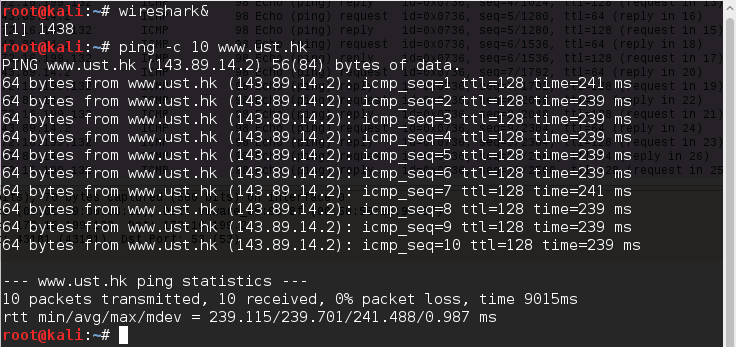
\includegraphics[width=\textwidth,height=\textheight,keepaspectratio,scale=0.5=0.5]{ping}
\end{figure}

\begin{figure}[H]
	\caption{The first ICMP packet}
	\centering
	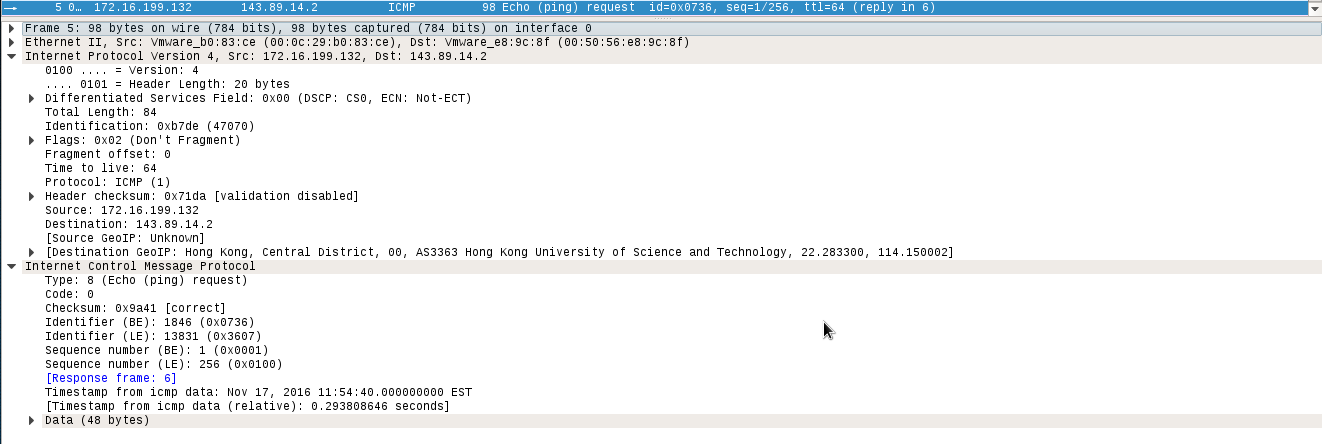
\includegraphics[width=\textwidth,height=\textheight,keepaspectratio,scale=0.5=0.5]{IMCP_pkt}
\end{figure}

\begin{figure}[H]
	\caption{The ICMP reply to the first packet}
	\centering
	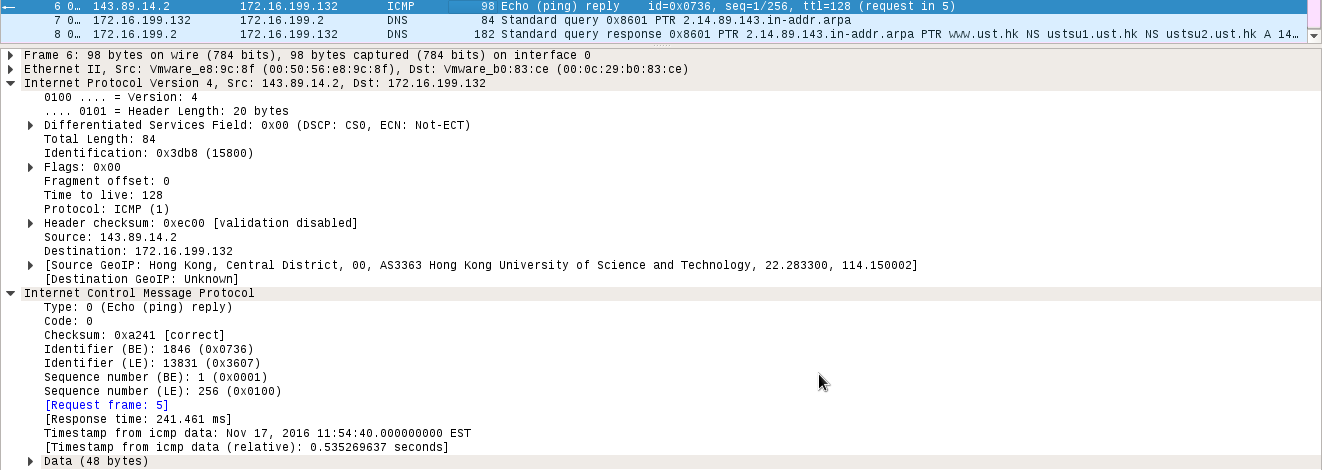
\includegraphics[width=\textwidth,height=\textheight,keepaspectratio,scale=0.5=0.5]{ICMP_reply}
\end{figure}

\subsection{ICMP and Traceroute}
\paragraph{Problem 1}
\begin{enumerate}[label=\textbf{Part \alph*)}, leftmargin=*, align=left]
	\item Host IP addr.: \texttt{172.16.199.132}.
	\item Dest IP addr.: \texttt{222.92.46.5}.
	\item UDP protocol No.: 17.
	\item TTL field value: 1
\end{enumerate}
\paragraph{Problem 2}
The fourth UDP packet had a TTL of 2.
\paragraph{Problem 3}
The ICMP TTL-exceeded error has type 11, code 0 field values

\paragraph{Problem 4}
??

\begin{figure}[H]
	\caption{The first UDP packet}
	\centering
	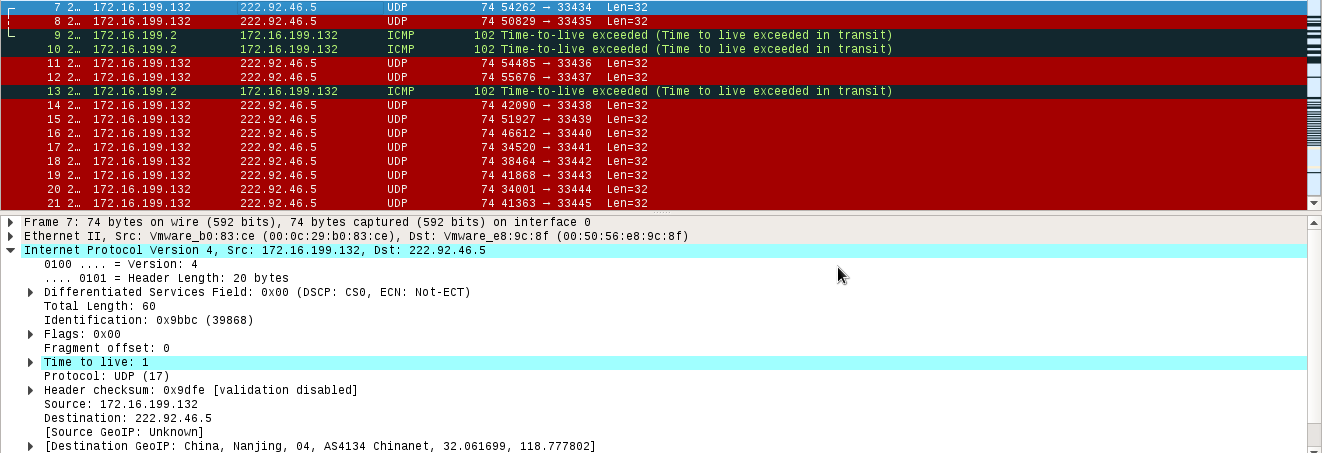
\includegraphics[width=\textwidth,height=\textheight,keepaspectratio,scale=0.5=0.5]{firstUDP}
\end{figure}

\begin{figure}[H]
	\caption{The fourth UDP packet}
	\centering
	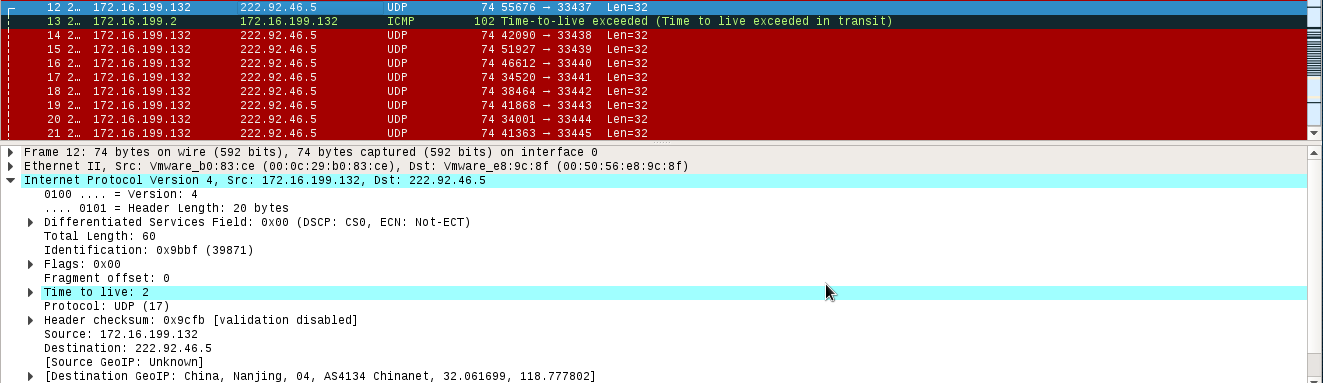
\includegraphics[width=\textwidth,height=\textheight,keepaspectratio,scale=0.5=0.5]{4thUDP}
\end{figure}

\begin{figure}[H]
	\caption{The ICMP TTL-exceeded packet}
	\centering
	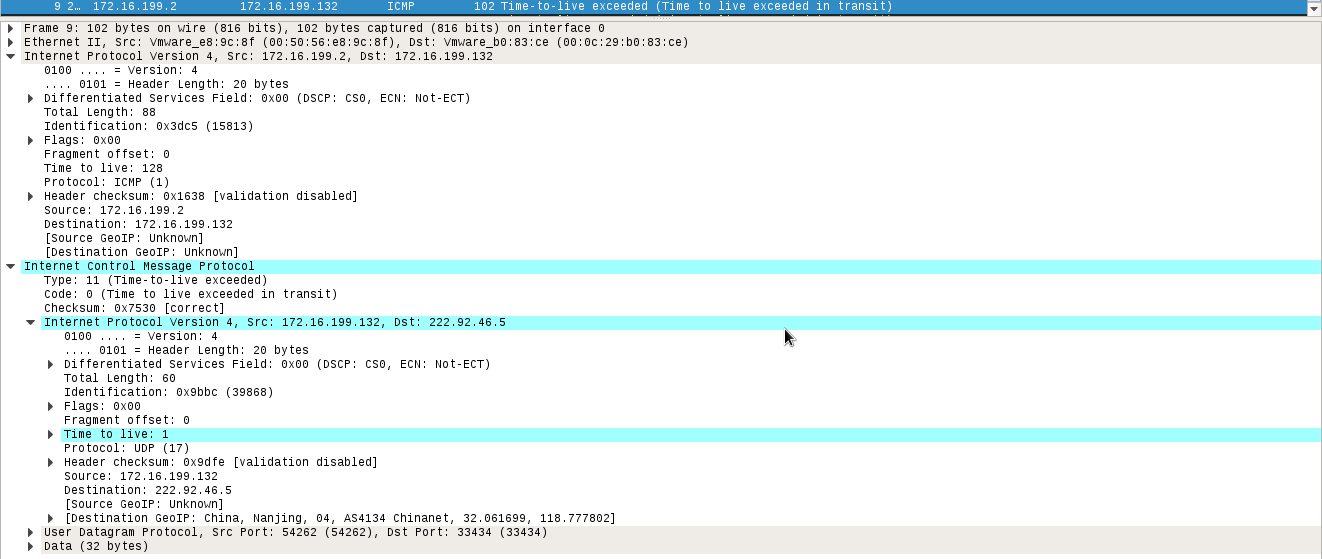
\includegraphics[width=\textwidth,height=\textheight,keepaspectratio,scale=0.5=0.5]{ttlexec}
\end{figure}

\begin{figure}[H]
	\caption{}
	\centering
	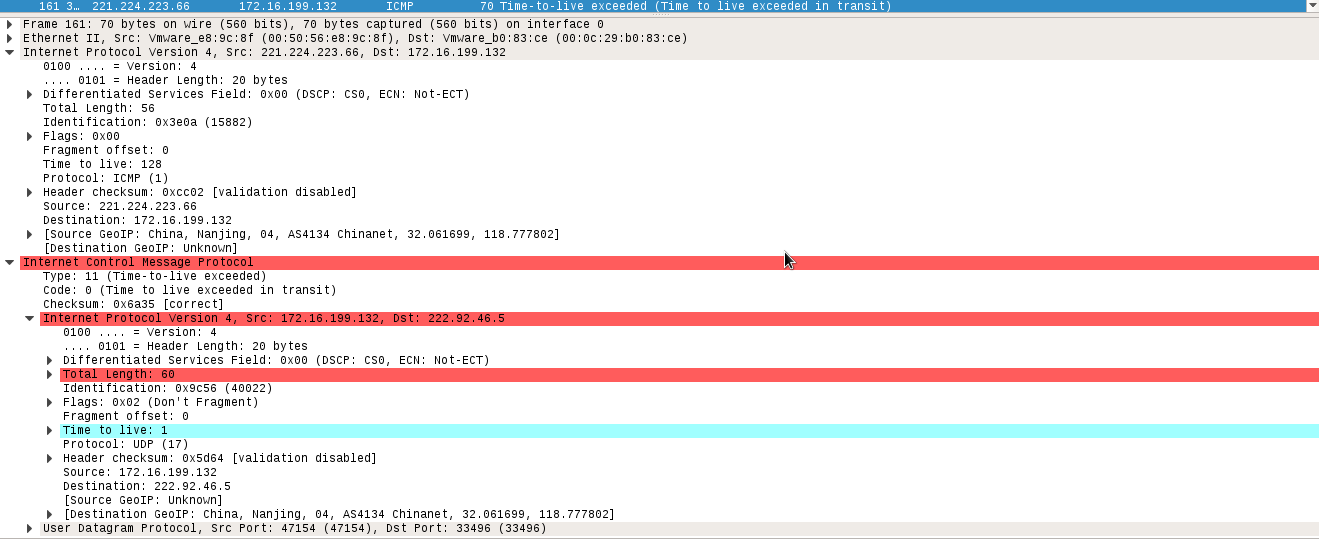
\includegraphics[width=\textwidth,height=\textheight,keepaspectratio,scale=0.5=0.5]{LastICMP}
\end{figure}

\subsection{Fragmentation}
\paragraph{Problem 1}
No fragrments and as no packet as the MF field set.
\paragraph{Problem 2}
Yes, the MF bit is set and the 1st packet. There are 2 fragments in the form of UDP packets
\paragraph{Problem 3}
Yes, there are 3 fragments.
\paragraph{Problem 4}
THe MF field is sen and the lenght of the packet is of maximum size. Also, the offset is 0.
\paragraph{Problem 5}
The MF field is 1 and the offset is 1480.
\paragraph{Problem 6}
The offset and the checksum.
\paragraph{Problem 7}
All Flags are set to 0 and the sum of the offset and packet length adds to the original datagram size.
\paragraph{Problem 8}
The MTU of the network is 1500 bytes.

\begin{figure}[H]
	\caption{Console output for ping with datagram of 1000B}
	\centering
	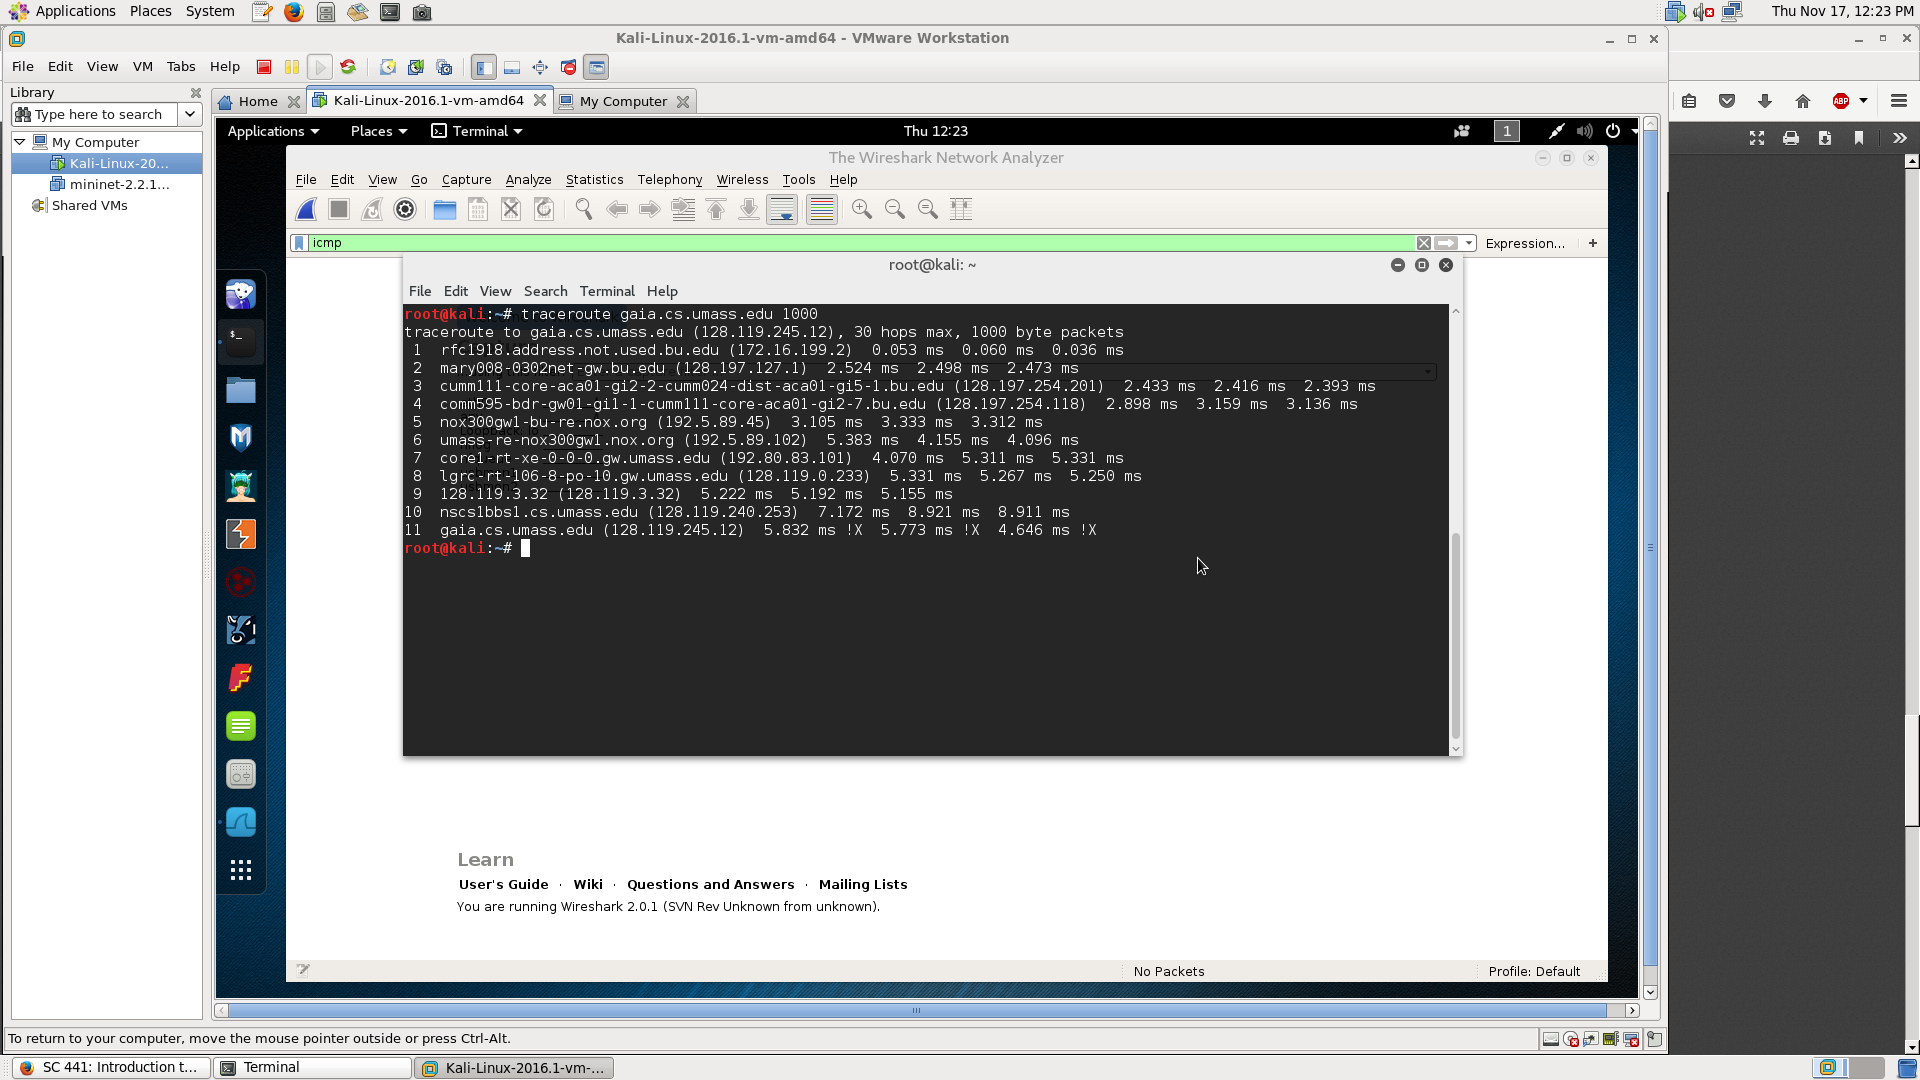
\includegraphics[width=\textwidth,height=\textheight,keepaspectratio,scale=0.5=0.5]{tr1000}
\end{figure}

\begin{figure}[H]
	\caption{Console output for ping with datagram of 2000B}
	\centering
	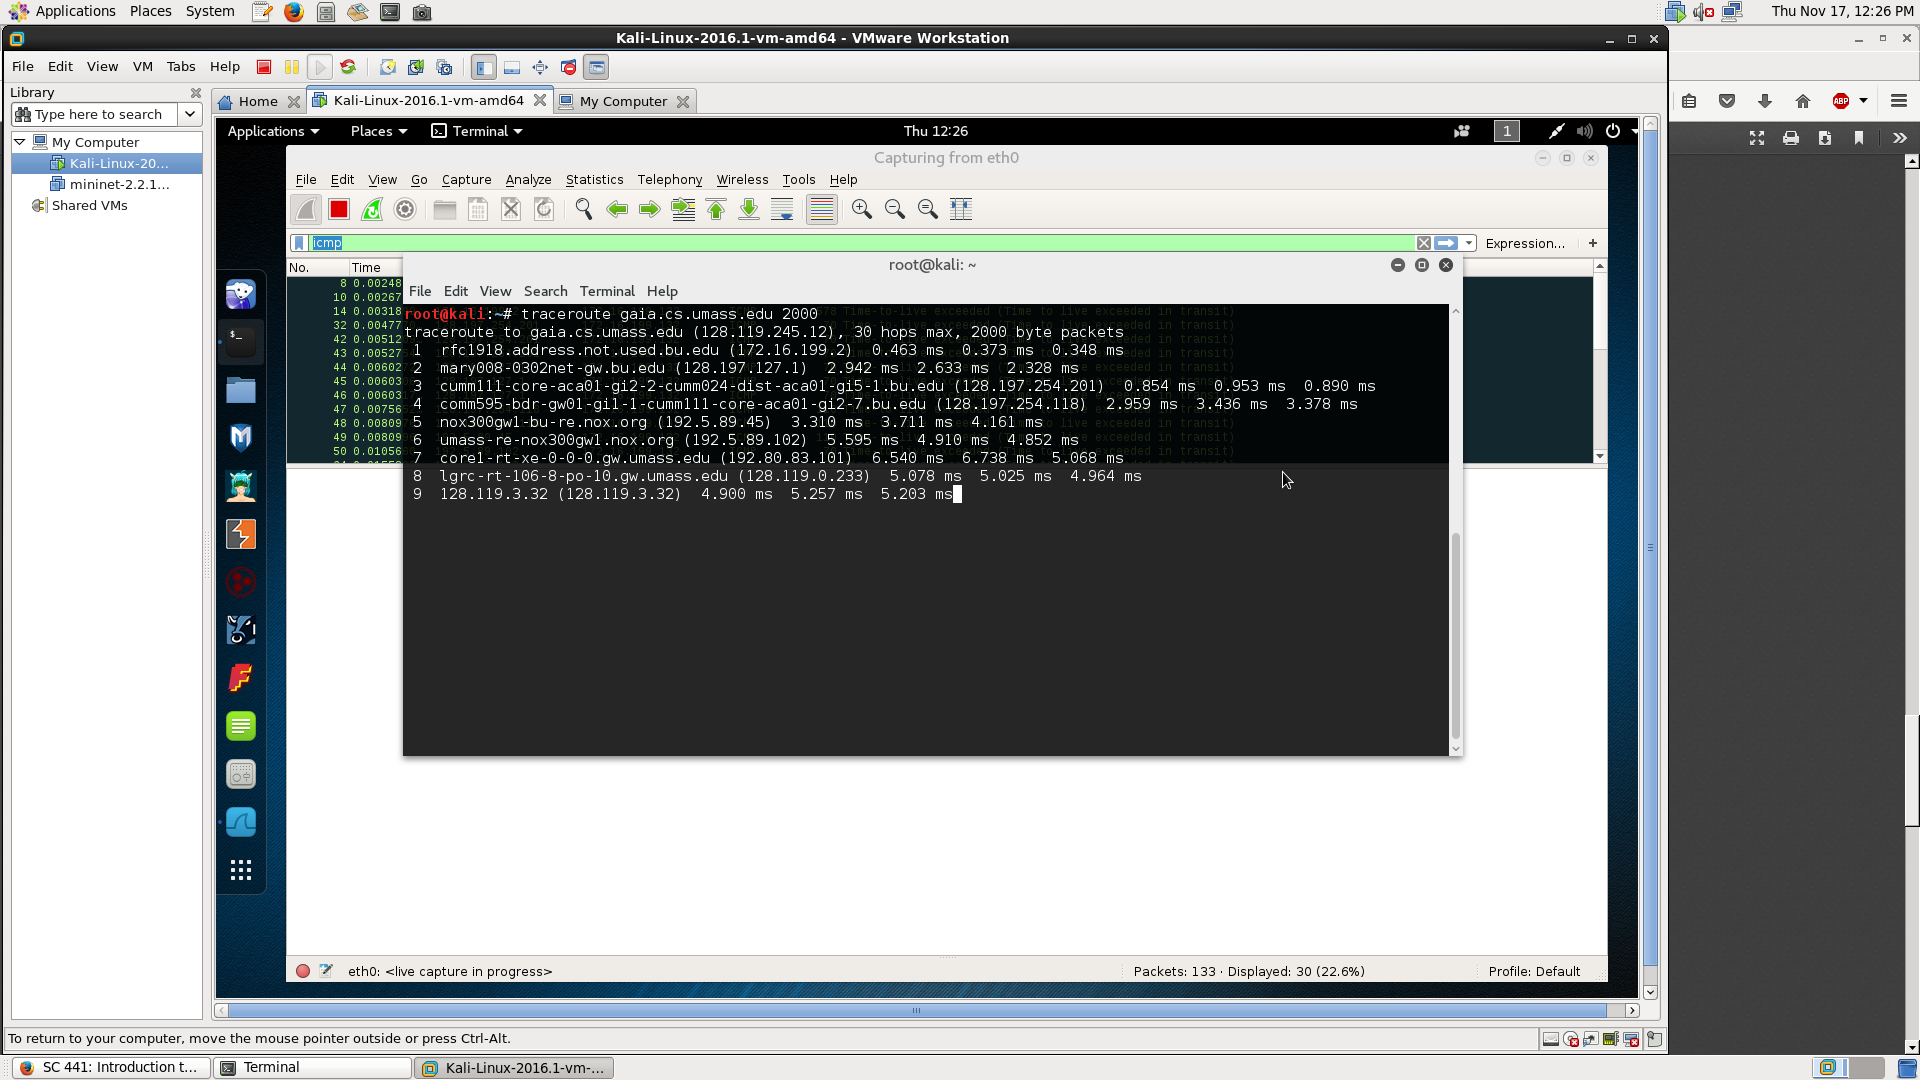
\includegraphics[width=\textwidth,height=\textheight,keepaspectratio,scale=0.5=0.5]{tr2000}
\end{figure}

\begin{figure}[H]
	\caption{Console output for ping with datagram of 3500B}
	\centering
	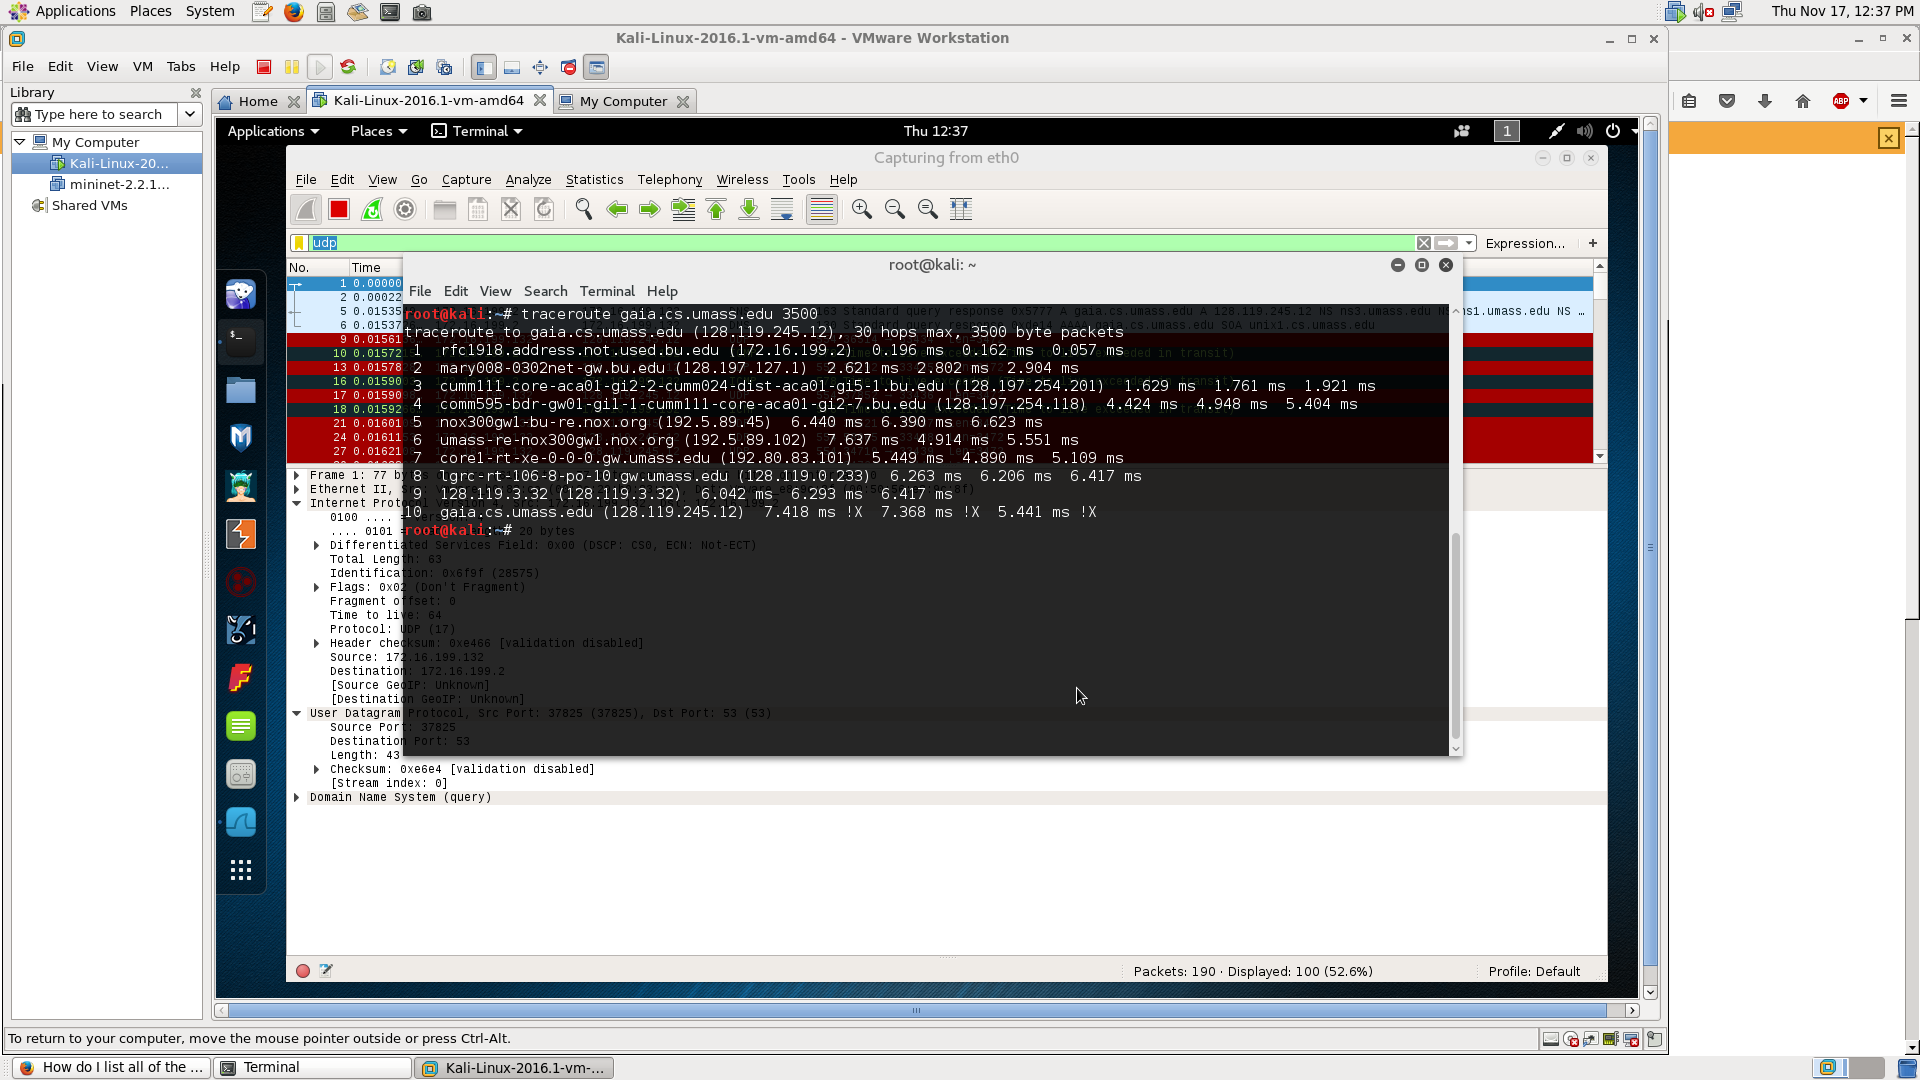
\includegraphics[width=\textwidth,height=\textheight,keepaspectratio,scale=0.5=0.5]{tr3500}
\end{figure}

\begin{figure}[H]
	\caption{First UDP probe}
	\centering
	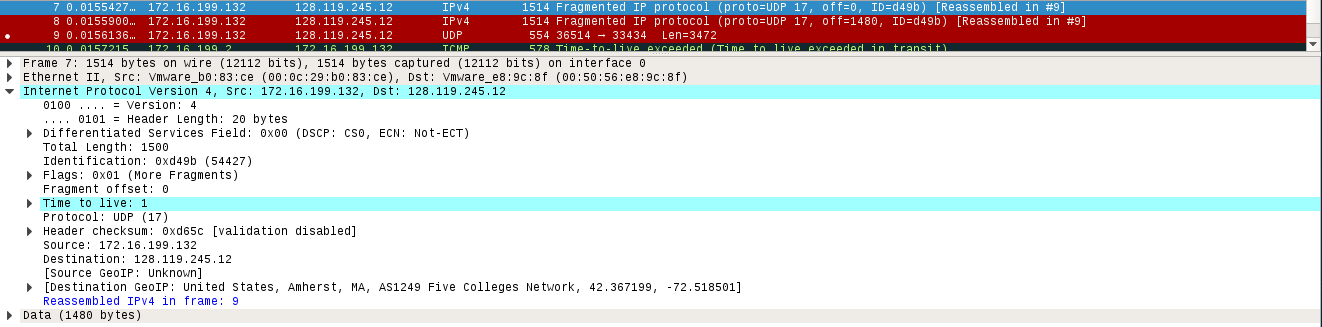
\includegraphics[width=\textwidth,height=\textheight,keepaspectratio,scale=0.5=0.5]{firstFrag}
\end{figure}

\begin{figure}[H]
	\caption{Second UDP fragment}
	\centering
	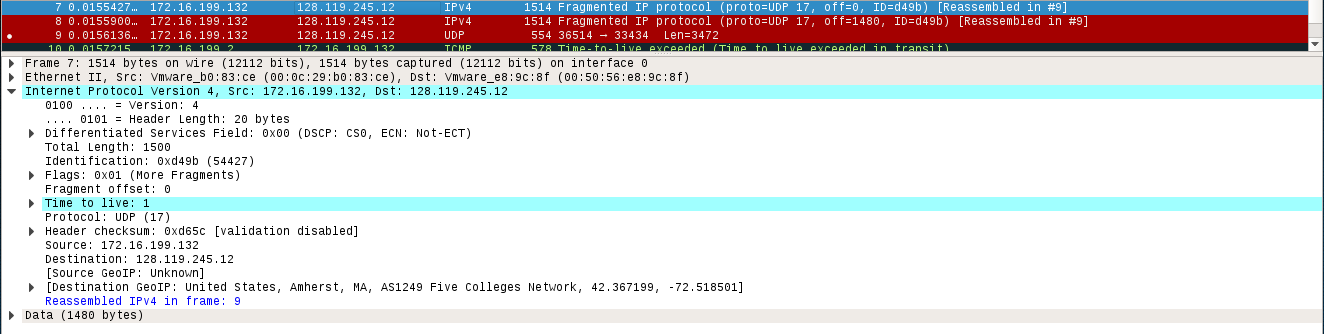
\includegraphics[width=\textwidth,height=\textheight,keepaspectratio,scale=0.5=0.5]{2ndFrag}
\end{figure}
\end{document}
This is never printed